\documentclass[]{article}

\usepackage{graphicx} %for å inkludere grafikk
\usepackage{verbatim} %for å inkludere filer med tegn LaTeX ikke liker
\usepackage{tabularx}
\usepackage{booktabs}
\usepackage{amsmath}
\usepackage{float}
\usepackage{color}
\usepackage{listings}
\usepackage{physics}
\usepackage{hyperref}
\usepackage{subfig}
\usepackage{mhchem}
\usepackage{natbib}
%opening
\title{}
\author{}

\begin{document}
	
\title{Fission: a TALYS report}
\author{Dorthea Gjestvang }
\date{December 2017}

\maketitle

\begin{abstract}

\end{abstract}

\section{Introduction}

\section{Theory}
\subsection{Fission barrier}
When observing the average binding energy per nucleon, as seen in Figure \ref{fig:binding_energy_per_nucleon}, one can see that for $A=$ the binding energy per A peaks, and then starts to decrease for increasing A. For nuclei situated to the right of this peak, it is thus possible to release energy by splitting in two lighter fragments, that is to fission. However, when studying the chart of nuclei shown in Figure \ref{fig:chart_of_nuclei}, we observe that very few nucley have spontaneous fission as their main decay mode. This is due to the so-called fission barrier.

\begin{figure}
	\centering
	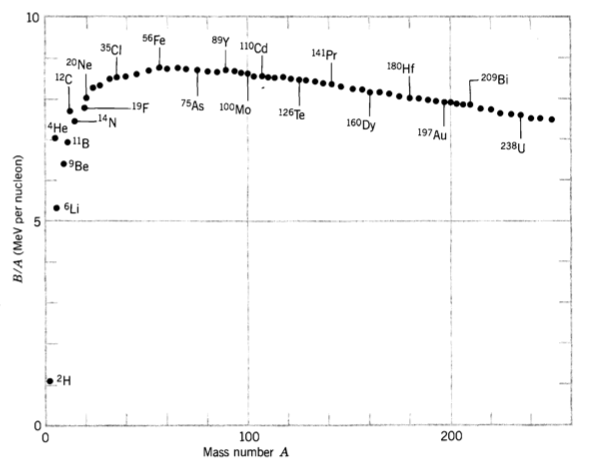
\includegraphics[scale=0.7]{binding_energy_per_nucleon.png}
	\caption{Average binding energy per nucleon. Figure from K.S. Krane p. }
	\label{binding_energy_per_nucleon}
\end{figure}



 In the liquid model, the fission barrier is described as a smooth, parabolic barrier, and is shown in Figure \ref{fig:smooth_fission_barrier}. It describes the energy needed to separate the two fission fragments as a function of separation distance. The fission barrier is due to both the nuclear force and the Coloumb force. A picture on why there is a fission barrier, is that in order for the two would-be fission fragments to separate, they have to get out of the potential well that is the nuclear force, and then pass the Coloumb barrier surrounding the nucleus. Thus energy must be applied for the fragments to be able to separate. This energy needed is often referred to as the activation energy, and is shown in Figure \ref{fig:smooth_fission_barrier} as the difference in energy between the ground state of the nucleus, and the maximum of the fission barrier potential. 

\subsection{The role of fission in nucleosynthesis}


\section{Method}


\section{Results}

\section{Discussion}

\section{Conclusion}


\bibliographystyle{plain}
\bibliography{TALYS.bib} 






\end{document}
